\section{Введение}
\subsection{Цели работы} 
\begin{itemize}
    \item изучение дифракции света на синусоидальной акустической решётке и наблюдение фазовой решётки методом тёмного поля.
\end{itemize}

\subsection{Используемые приборы}
\begin{itemize}
    \item оптическая скамья, осветитель, два длиннофокусных объектива, кювета с жидкостью, кварцевый излучатель с микрометрическим винтом, генератор ультразвуковой частоты, линза, вертикальная нить на рейтере, микроскоп.
\end{itemize}

\subsection{Теоретическая часть}

\subsubsection{Спектральный метод в оптике}

Спектральный метод позволяет представить сложные оптические явления через суперпозицию простых волн. В случае дифракции света это даёт возможность описать распространение волн через разложение волнового поля на плоские волны различных направлений.

Основное преимущество спектрального метода заключается в том, что каждая элементарная плоская волна при распространении приобретает свой фазовый набег, зависящий от её пространственной частоты. В результате интерференции этих волн формируется наблюдаемая дифракционная картина.

\subsubsection{Дифракция на фазовой синусоидальной решётке}

В данной работе изучается дифракция света на ультразвуковой волне в жидкости. Ультразвуковая волна создаёт периодические изменения показателя преломления среды, формируя фазовую синусоидальную решётку.

Функция пропускания такой решётки имеет вид:
\begin{equation}
    t(x) = e^{im \cos \Omega x}
\end{equation}
где $m$ — глубина модуляции фазы (обычно мала), $\Omega$ — пространственная частота решётки.

При малой глубине модуляции ($m \ll 1$) функцию пропускания можно представить как:
\begin{equation}
    t(x) \approx 1 + im\cos\Omega x = 1 + \frac{im}{2}e^{i\Omega x} + \frac{im}{2}e^{-i\Omega x}
\end{equation}

При освещении решётки плоской волной формируется три компоненты:
\begin{equation}
    f(x,z) = ae^{ikz} + \frac{iam}{2}e^{i(\Omega x + \sqrt{k^2-\Omega^2}z)} + \frac{iam}{2}e^{i(-\Omega x + \sqrt{k^2-\Omega^2}z)}
\end{equation}

Эти компоненты соответствуют центральному (нулевому) и двум боковым (±1) дифракционным максимумам. Особенность фазовой решётки заключается в том, что дифрагированные волны сдвинуты по фазе на $\pi/2$ относительно центральной волны.

\subsubsection{Метод тёмного поля}

Для визуализации фазовых объектов, которые не изменяют амплитуду проходящей волны, а только её фазу, используются специальные методы, один из которых — метод тёмного поля, предложенный Цернике.

При прохождении плоской волны через фазовый объект (например, акустическую решётку в жидкости) входное поле можно представить в виде:

\begin{equation}
    f_0(x) = e^{im \cos \Omega x} \approx 1 + im \cos \Omega x = 1 + \frac{im}{2}e^{i\Omega x} + \frac{im}{2}e^{-i\Omega x}
\end{equation}

где $m \ll 1$ — глубина фазовой модуляции.

Таким образом, входное поле представляется в виде суммы трёх компонентов:
\begin{itemize}
    \item Прямое (нулевой порядок) — плоская волна единичной амплитуды $f_0(x) = 1$
    \item Две наклонные волны (первые порядки дифракции) с амплитудой $m/2$, пространственными частотами $\pm\Omega$ и фазовым сдвигом $\pi/2$ относительно основной волны
\end{itemize}

\begin{figure}[htbp]
    \centering
    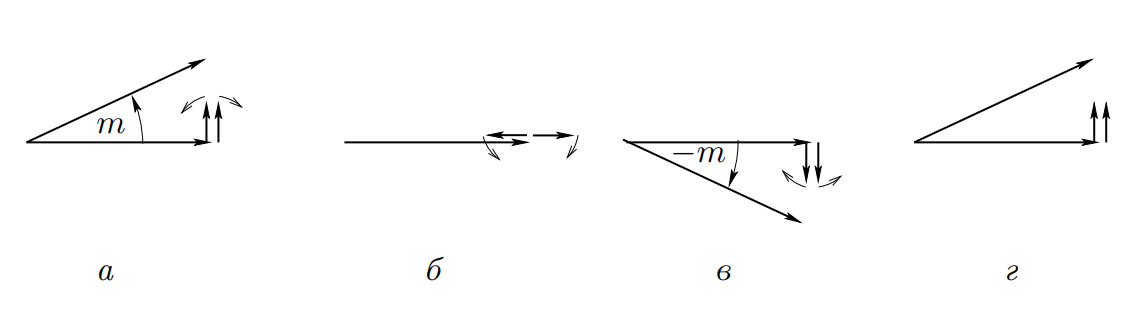
\includegraphics[width=0.8\textwidth]{pictures/phase_grid_vectors.png}
    \caption{Векторные диаграммы для фазовой решётки}
    \label{fig:phase_grid_vectors}
\end{figure}

В методе тёмного поля в фурье-плоскости оптической оси устанавливается непрозрачный экран (диафрагма), который блокирует прохождение прямой (осевой) волны. В результате в плоскости изображения интерферируют только дифрагированные волны.

При таком методе наблюдения поле в выходной плоскости имеет вид:
\begin{equation}
    f(x) = \frac{im}{2}e^{i\Omega x} + \frac{im}{2}e^{-i\Omega x} = im \cos \Omega x
\end{equation}

Распределение интенсивности в плоскости изображения:
\begin{equation}
    I(x) = |f(x)|^2 = m^2 \cos^2 \Omega x
\end{equation}

Характерной особенностью метода тёмного поля является удвоение частоты наблюдаемой структуры — расстояние между тёмными полосами соответствует смещению на $\Lambda/2$, где $\Lambda = 2\pi/\Omega$ — период решётки.

Метод тёмного поля аналогичен методу, который в радиотехнике используется для преобразования фазовой модуляции в амплитудную и называется "приёмом без несущей".

\subsubsection{Экспериментальная установка}

\subsubsection*{Схема экспериментальной установки}

\begin{figure}[htbp]
    \centering
    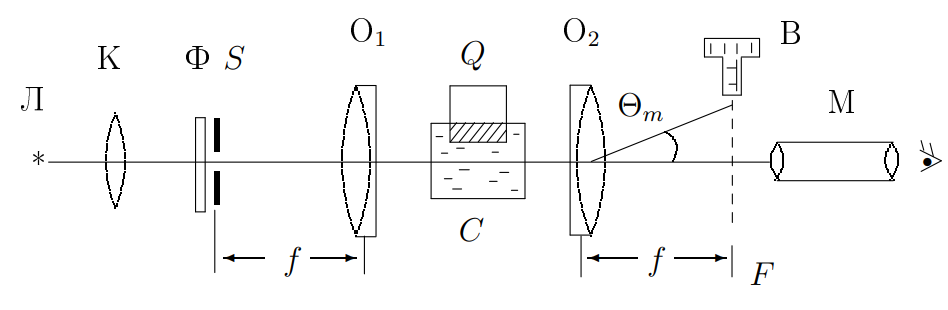
\includegraphics[width=0.8\textwidth]{pictures/setup.png}
    \caption{Схема экспериментальной установки для наблюдения дифракции на акустической решётке}
    \label{fig:setup}
\end{figure}

Экспериментальная установка (рис.~\ref{fig:setup}) состоит из источника света Л с конденсором К, монохроматора с входной щелью S и светофильтром Ф, коллиматорного объектива O$_1$, кюветы с водой C, в которую погружён ультразвуковой излучатель Q, камерного объектива O$_2$ и экрана с микроскопом M для наблюдения дифракционной картины.

Ультразвуковой излучатель создаёт в кювете синусоидальную акустическую волну, которая модулирует показатель преломления среды, образуя фазовую дифракционную решётку. При определённых положениях излучателя в кювете формируется стоячая волна, что делает возможным наблюдение дифракционной картины.

\begin{figure}[htbp]
    \centering
    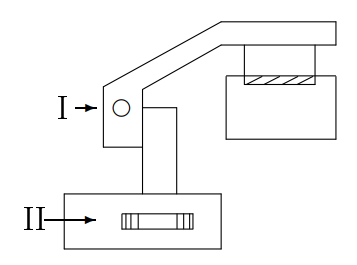
\includegraphics[width=0.6\textwidth]{pictures/device.png}
    \caption{Устройство для перемещения излучателя}
    \label{fig:device}
\end{figure}

Точное вертикальное позиционирование излучателя обеспечивается механизмом с винтами грубой (I) и точной (II) подачи (рис.~\ref{fig:device}). Это позволяет настраивать условия образования стоячей волны в кювете.

Для измерения параметров дифракционной картины в фокальной плоскости F объектива O$_2$ установлено стекло с измерительной шкалой, перемещаемое микрометрическим винтом B. На стекле нанесены реперная линия, перекрестие и проволока (рис.~\ref{fig:reticle}).

\begin{figure}[htbp]
    \centering
    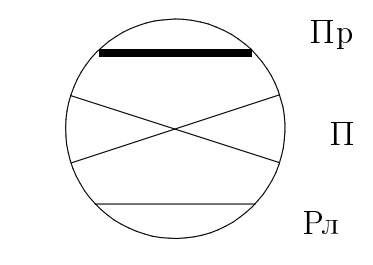
\includegraphics[width=0.5\textwidth]{pictures/reticle.png}
    \caption{Проволока Пр, перекрестие П и реперная линия — в фокальной плоскости объектива О$_2$}
    \label{fig:reticle}
\end{figure}

Длина ультразвуковой волны $\Lambda$ определяется из условия дифракции:
\begin{equation}
    \Lambda\sin\Theta_m = m\lambda
\end{equation}

Для малых углов дифракции это выражение упрощается:
\begin{equation}
    l_m = m\frac{f\lambda}{\Lambda}
\end{equation}
где $l_m$ — расстояние между m-м и нулевым максимумами, $f$ — фокусное расстояние объектива O$_2$, $\lambda$ — длина волны света.

Скорость звука в воде вычисляется по формуле:
\begin{equation}
v = \Lambda\nu
\end{equation}
где $\nu$ — частота ультразвукового излучателя.

\subsubsection*{Наблюдение акустической решётки методом тёмного поля}

\begin{figure}[htbp]
    \centering
    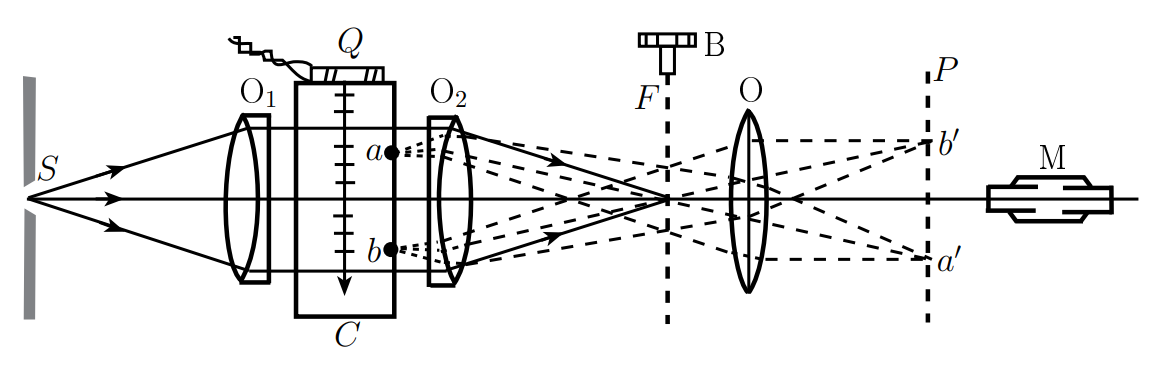
\includegraphics[width=0.8\textwidth]{pictures/dark_field.png}
    \caption{Наблюдение акустической решётки методом тёмного поля}
    \label{fig:dark_field}
\end{figure}

Метод тёмного поля (рис.~\ref{fig:dark_field}) позволяет наблюдать фазовые объекты, которые невидимы в обычных оптических системах. Суть метода заключается в устранении центрального (нулевого) дифракционного максимума с помощью непрозрачного экрана. В результате изображение формируется только дифрагированными лучами, несущими информацию о фазовых неоднородностях объекта.

Характерная особенность метода — удвоение числа наблюдаемых деталей структуры. Расстояние между тёмными полосами соответствует смещению в плоскости кюветы на $\Lambda/2$. 

Этот метод эффективен только для стоячих волн, так как в случае бегущей волны фазовые неоднородности перемещаются слишком быстро для визуального наблюдения.